\documentclass{article}
\usepackage{graphicx} % Required for inserting images
\documentclass{article}
\usepackage{graphicx} % 插入图片所需的宏包


\title{\textbf{Research on Multi-Criteria Scheduling Strategies for Heterogeneous Kubernetes Clusters}}
\author{Sun Guifa,Sun jianpeng,Xie xiguo}

\newpage
\begin{document}

\maketitle
\newpage
\section{Introduction}
\subsection{Research Background}
Efficient utilization of node resources and reduction of job waiting time in heterogeneous clusters are key to improving overall cluster resource utilization. Kubernetes is the leading system in the field of container orchestration. However, its default CPU and memory scheduling mechanisms are insufficient for handling jobs that require multiple resources. Therefore, integrating a multi-criteria scheduling algorithm that combines the Analytic Hierarchy Process (AHP) with bin-packing strategies can effectively reduce job waiting times caused by resource fragmentation.
\subsection{Problem Statement}
\begin{itemize}
  \item In addition to traditional resource metrics such as CPU and memory, the approach also incorporates a variety of other resource indicators, including storage, GPU-like accelerator cards, and container images.
  \item It not only requires objective metrics, but also integrates users' subjective preferences with objective indicators, enabling the selection of appropriate nodes for scheduling through multi-node decision-making.
\end{itemize}

\subsection{Research objectives and significance}
This paper takes into account the measurement of resource metrics and incorporates users’ subjective decision-making by integrating the Analytic Hierarchy Process (AHP) for scheduling computation. As a result, it significantly reduces Pod scheduling latency and improves overall cluster resource utilization.

\section{Methodology}
\subsection{Overall system architeture}

\newpage
\begin{figure}[htbp]
  \centering
  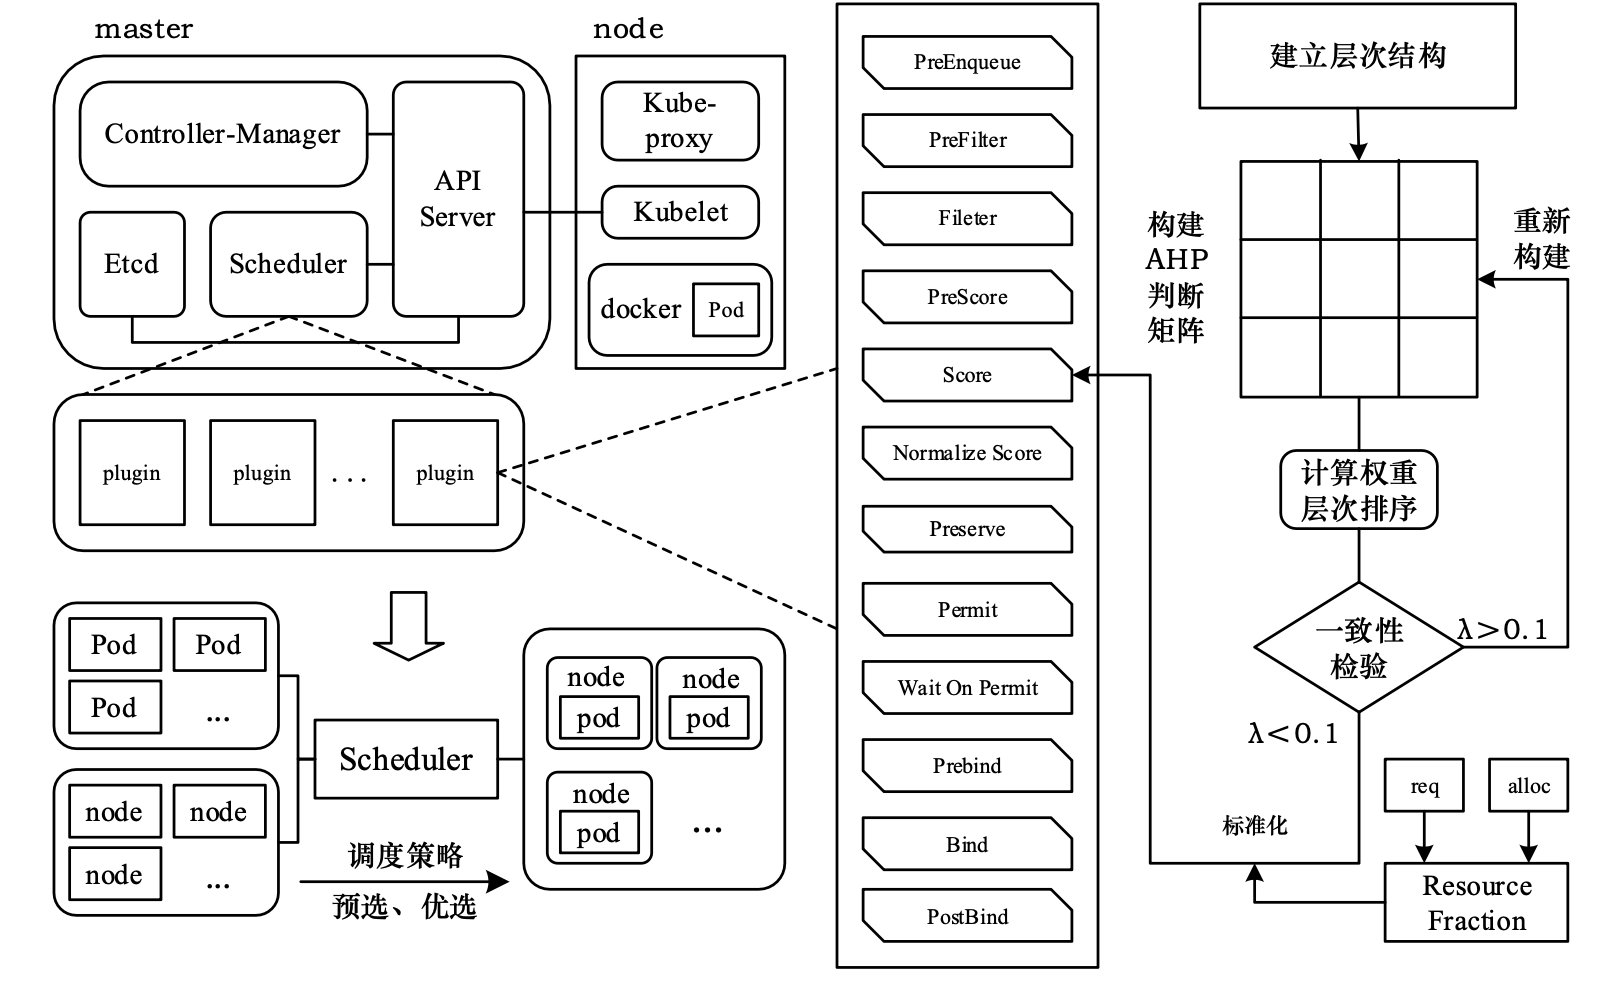
\includegraphics[width=0.65\textwidth]{pic01.png} % 图片文件名,不需要加扩展名
  \caption{Overall system architeture}
  \label{1}
\end{figure}

\subsection{Kubernetes Scheduling Framework}
\begin{figure}[htbp]
  \centering
  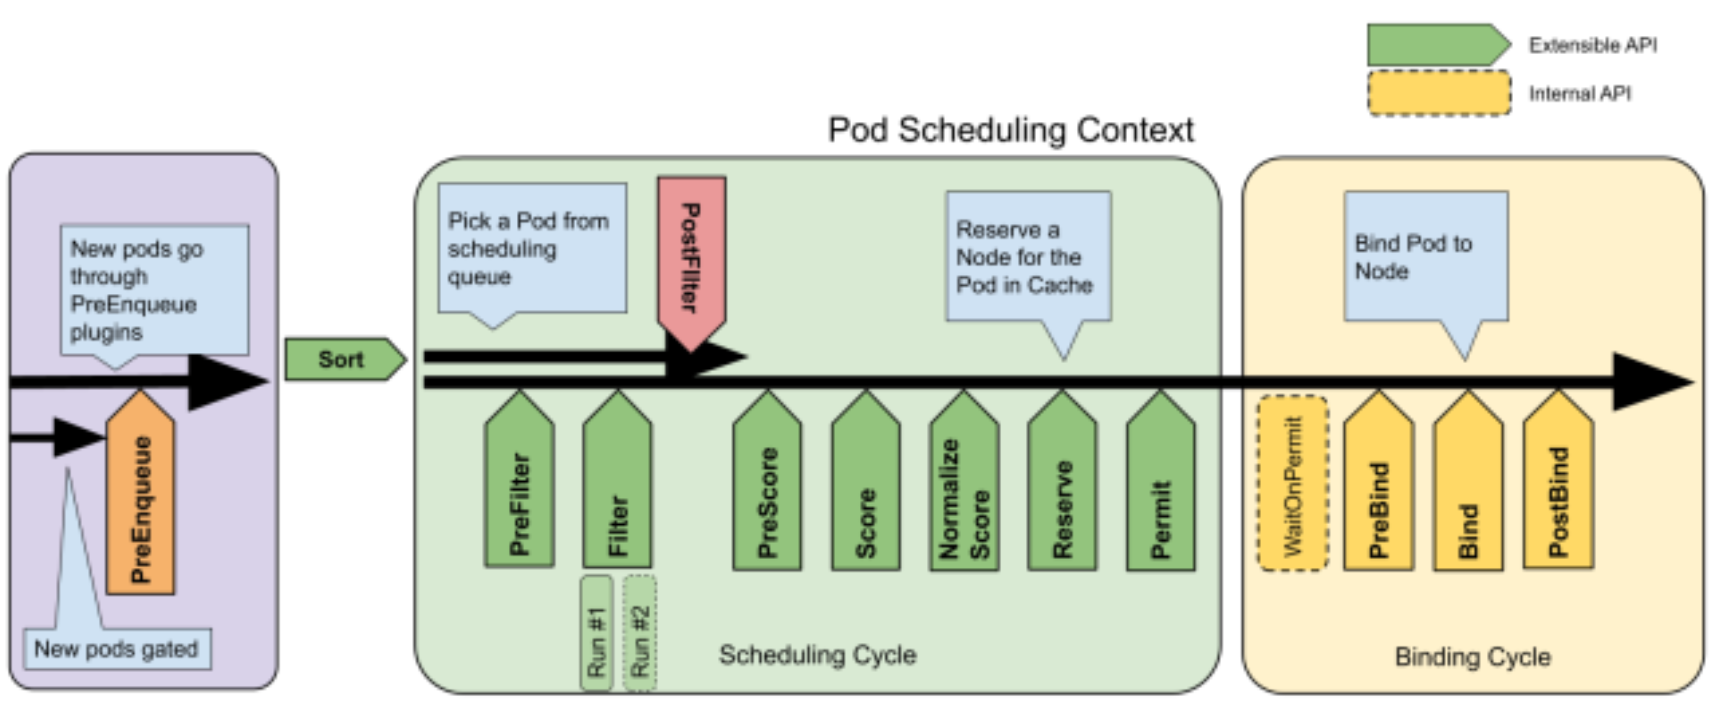
\includegraphics[width=0.65\textwidth]{pic02.png} % 图片文件名,不需要加扩展名
  \caption{Kubernetes Scheduling Framework}
  \label{2}
\end{figure}
The Kubernetes scheduling framework is a plugin architecture designed for the Kubernetes scheduler. It consists of a set of plugin APIs that are compiled directly into the scheduler, enabling the core scheduling logic to remain simple and maintainable. Once registered, scheduler plugins are invoked at one or more extension points. Some of these plugins are used to provide information, while others can influence or alter scheduling decisions.

\subsection{Packing and Load Balancing Scheduling}
\newpage
\begin{figure}[htbp]
  \centering
  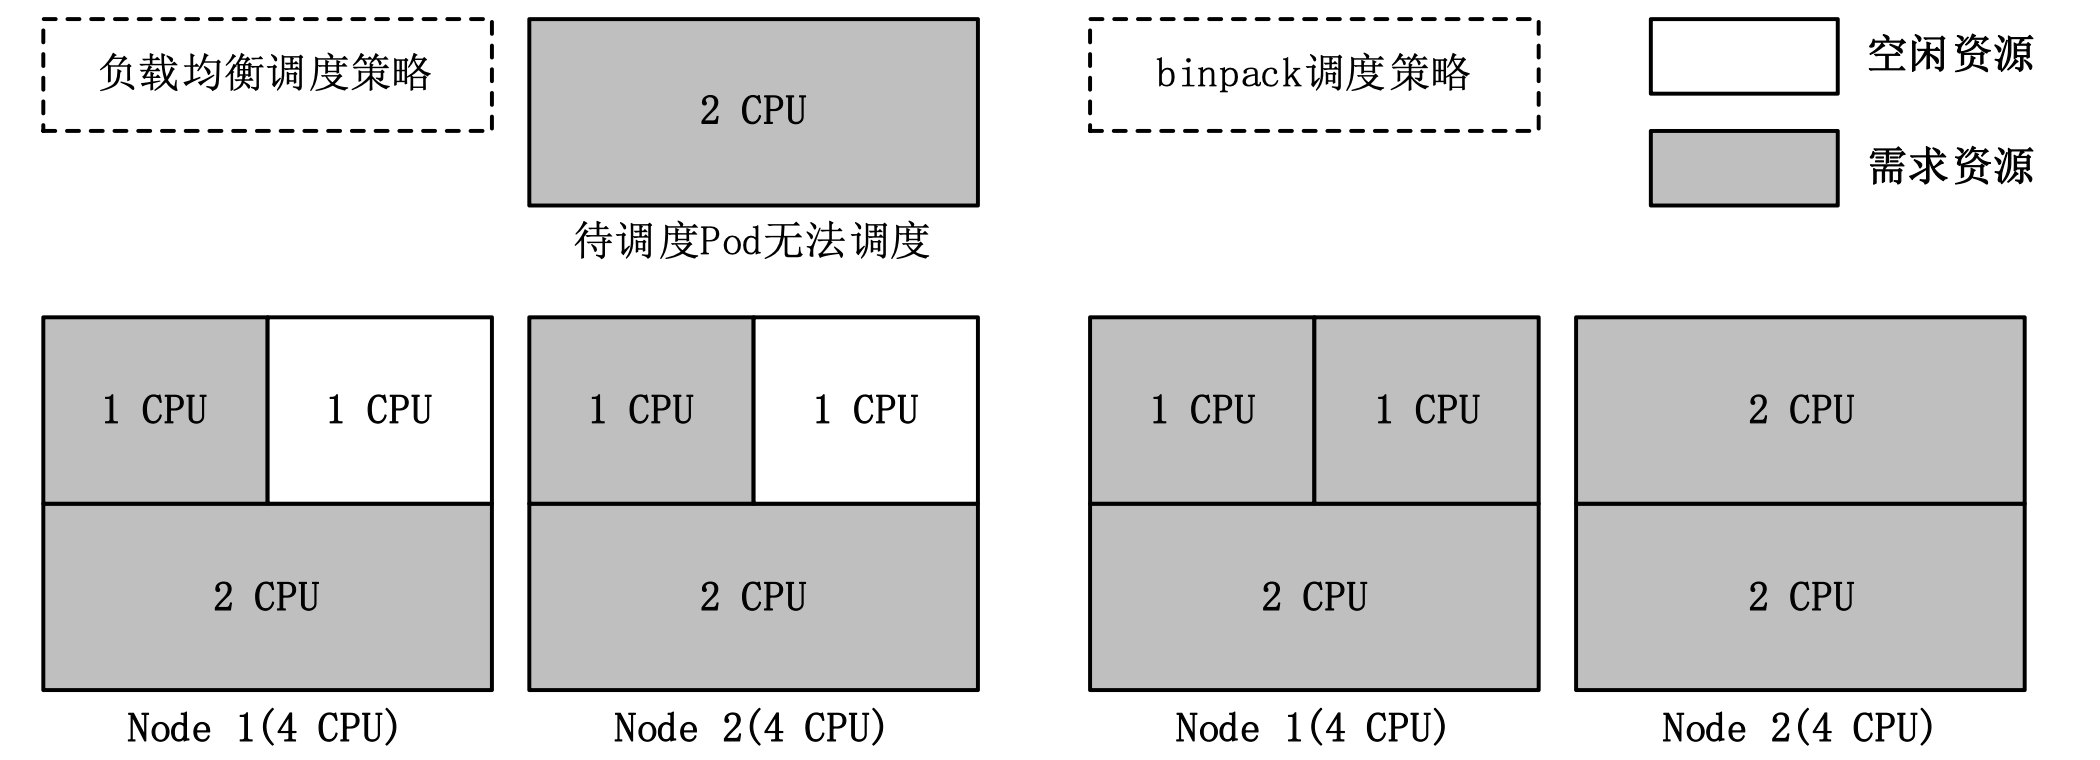
\includegraphics[width=0.65\textwidth]{pic03.png} % 图片文件名,不需要加扩展名
  \caption{Packing and Load Balancing Scheduling}
  \label{3}
\end{figure}
Bin-packing scheduling is a strategy that focuses on maximizing resource utilization. It tends to assign pending jobs to the nodes with the highest current resource usage. By compactly placing workloads, the scheduler can pack more jobs into the cluster, thereby improving overall resource efficiency.

\subsection{Analytic Hierarchy Process}
\subsubsection{Scheduling Hierarchy}
\begin{figure}[htbp]
  \centering
  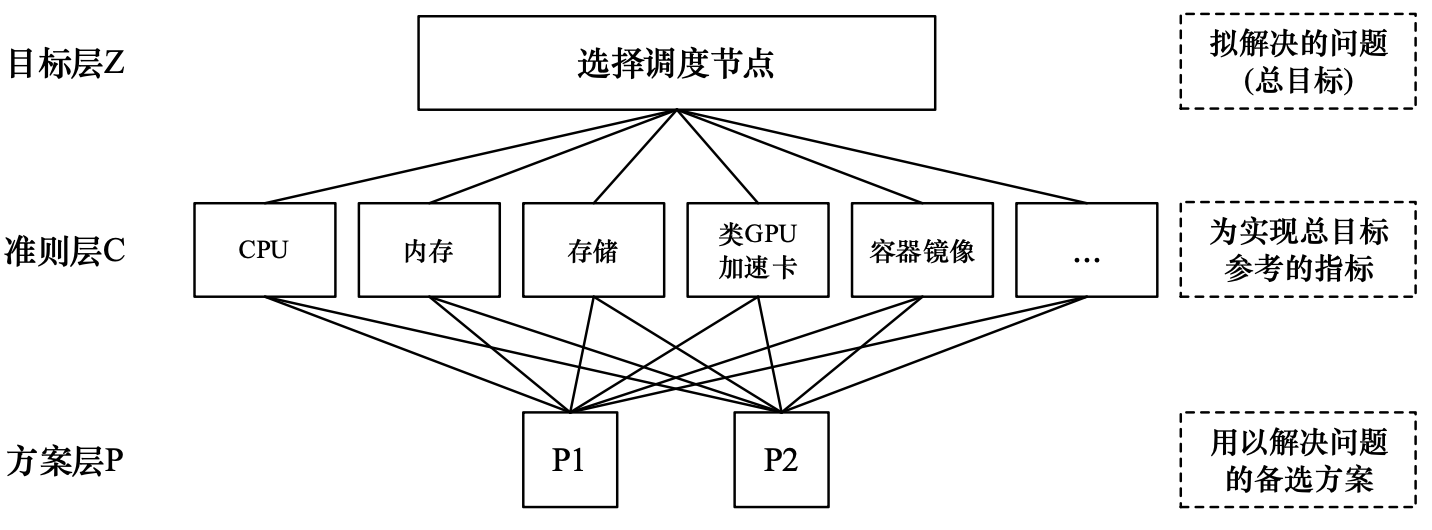
\includegraphics[width=0.65\textwidth]{pic04.png} % 图片文件名,不需要加扩展名
  \caption{Scheduling Hierarchy}
  \label{4}
\end{figure}
The Analytic Hierarchy Process (AHP) divides the decision-making problem into three hierarchical levels: the **goal level (Z)**, the **criteria level (C)**, and the **alternative level (P)**. In the context of job scheduling research for Kubernetes clusters on large-scale heterogeneous computing platforms, a hierarchical structure is constructed with **five resource indicators** at the criteria level to serve as evaluation metrics for scheduling decisions.
\subsubsection{Judgment Matrix}
\newpage
\begin{figure}[htbp]
  \centering
  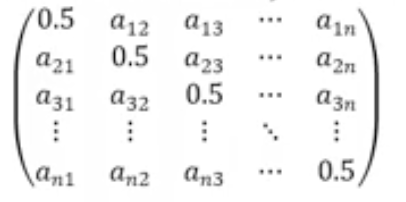
\includegraphics[width=0.65\textwidth]{pic05.png} % 图片文件名,不需要加扩展名
  \caption{Matrix}
  \label{5}
\end{figure}

\begin{figure}[htbp]
  \centering
  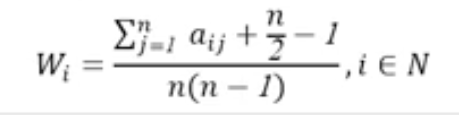
\includegraphics[width=0.65\textwidth]{pic06.png} % 图片文件名,不需要加扩展名
  \caption{Caculate Wi}
  \label{6}
\end{figure}

\begin{figure}[htbp]
  \centering
  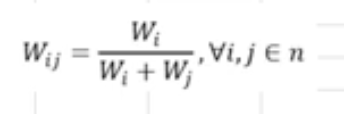
\includegraphics[width=0.65\textwidth]{pic07.png} % 图片文件名,不需要加扩展名
  \caption{Caculate Wij}
  \label{7}
\end{figure}


\subsubsection{Priority Vector and Consistency Check}
\newpage
\begin{figure}[htbp]
  \centering
  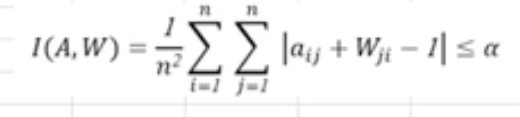
\includegraphics[width=0.65\textwidth]{pic08.png} % 图片文件名,不需要加扩展名
  \caption{Consistency Check}
  \label{7}
\end{figure}

\subsection{Kube-schedular settings}



\subsection{Description of models, algorithms, or frameworks used}
\subsection{Key implementation details}
\subsection{Algorithm derivation or process flow}

\section{Experiments and Evaluation}
\subsection{Description of experimental environment and datasets}
\subsection{Experiment setup and parameter configuration}
\subsection{Comparison with baseline or existing methods}
\subsection{Result analysis and visualization}

\section{Conclusion and Future Work}
\subsection{Summary of main work and contributions}
\subsection{Existing limitations and challenges}
\subsection{Future research directions}





\end{document}
